
\section{Figures and visual evidence}
\begin{figure}[h]\centering
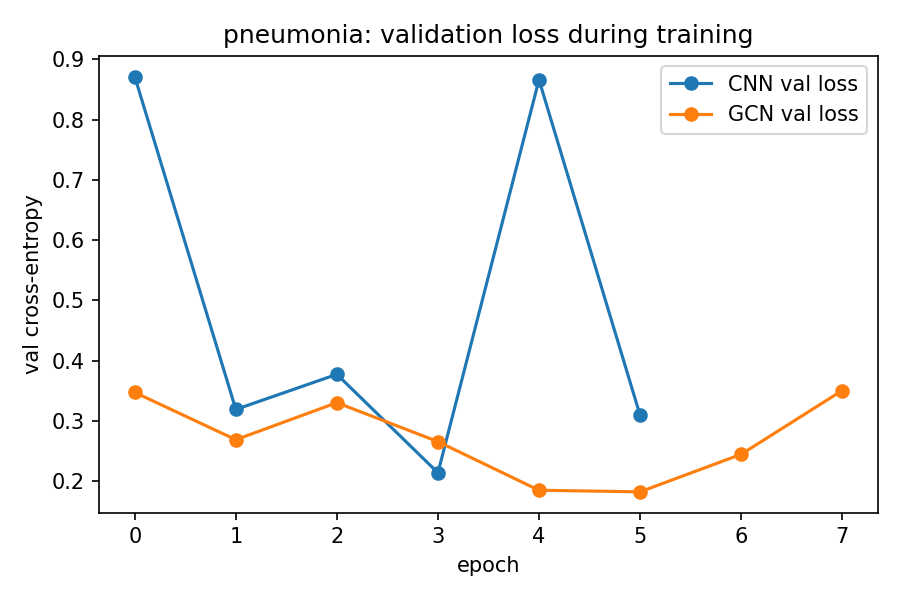
\includegraphics[width=0.72\textwidth]{../figures/pneumonia_training_curves.png}
\caption{Pneumonia baseline training and validation loss, CNN core vs
RegionGCN hybrid (committed history in
\texttt{results/pneumonia/baseline\_results.json}).}
\end{figure}
\begin{figure}[h]\centering
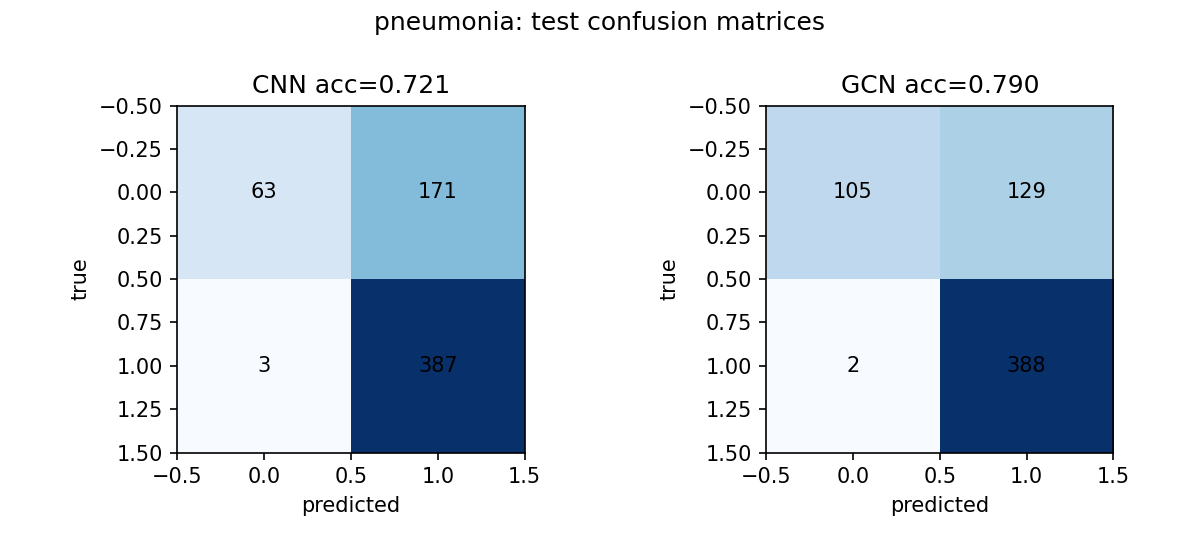
\includegraphics[width=0.6\textwidth]{../figures/pneumonia_confusion.png}
\caption{Pneumonia test-set confusion, RegionGCN (624 held-out official
test images). Sensitivity is near-perfect; errors concentrate on the
normal class.}
\end{figure}
\begin{figure}[h]\centering
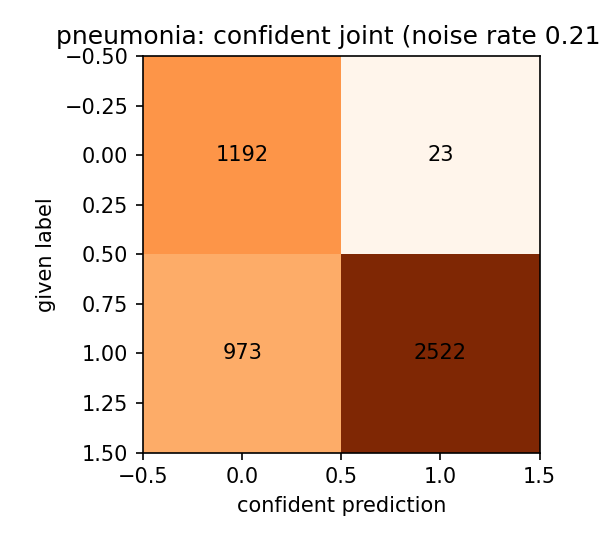
\includegraphics[width=0.62\textwidth]{../figures/pneumonia_confident_joint.png}
\caption{Pneumonia confident joint from the 3-fold out-of-fold census.
The off-diagonal mass is again strongly one-directional: 973 training
images labelled \emph{pneumonia} cross-validate as \emph{normal}, vs 23
in the opposite direction.}
\end{figure}
\begin{figure}[h]\centering
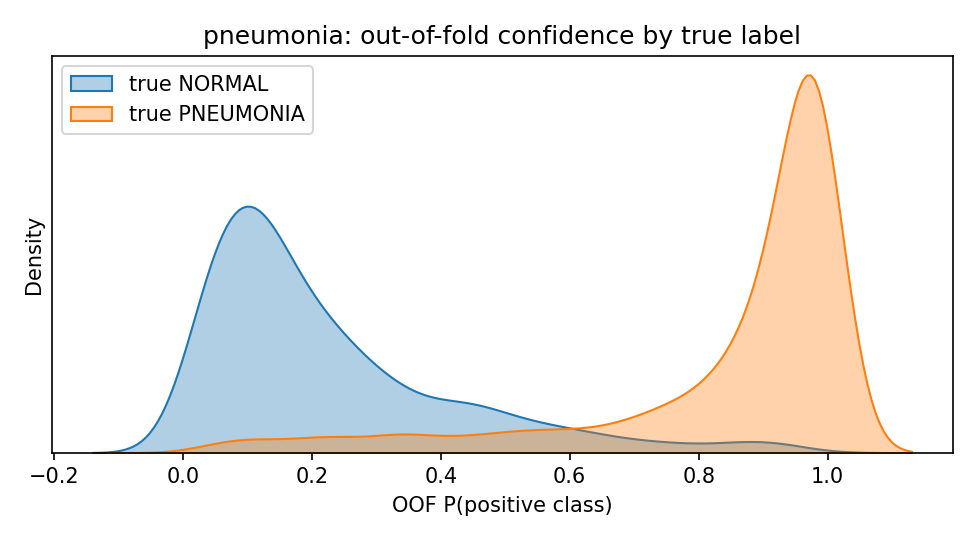
\includegraphics[width=0.62\textwidth]{../figures/pneumonia_oof_distributions.png}
\caption{Out-of-fold confidence by true label (seaborn KDE):
PNEUMONIA-labelled films with near-zero pneumonia confidence form the
heavy wrong-side tail.}
\end{figure}

\section{Interpretability}
\subsection{Flagged-image forensics}
Flagged films are measurably atypical in sharpness, contrast, and entropy
(\texttt{results/pneumonia/flagged\_image\_properties.json}; per-image rows
in \texttt{results/flagged\_property\_rows.csv}). Grad-CAM attribution for
the pneumonia models is produced in the interpretability battery
(SimpleITK/grad-cam stage) and reported with its committed evidence.
\subsection{Calibration}
Because the class-weighted tuned configuration shifts the decision
threshold implicitly, we report sensitivity/specificity pairs for every
configuration rather than a single operating point, and the ROC-AUC as the
threshold-free summary.

\section{Discussion}
\subsection{What the census is and is not}
The census estimates \emph{statistical} label inconsistency: a film is
flagged when cross-validated confidence in the other class exceeds the
class-mean threshold. Flags are falsifiable per-identifier claims, not
expert-readability judgements; borderline films are expected to concentrate
in the flagged set.
\subsection{Removal helped pneumonia but not malaria - unattributed to labels}
Here the flag-removed RegionGCN gains +5.9 points over its own baseline, in contrast to the malaria regime --- but the random-removal control (GCN 82.77$\pm$1.93\% vs flagged 84.94\%) matches it, so the divergence cannot be credited to label quality; the regime analysis below is kept as hypothesis, explicitly not as conclusion. Two regime differences plausibly explain
the divergence: (i) the pneumonia census flags 21.15\% of training films
--- a far heavier contamination --- so removal eliminates genuinely
conflicting gradient signal rather than hard-but-correct examples; (ii)
the official test split is patient-level and was curated separately from
the training pool, so its label process is not the same contaminated
process. We report the contrast between the two diseases as a finding in
itself: the value of an annotation-consistency audit is regime-dependent, and the
regime variables (contamination mass, test-set curation) are measurable.
\subsection{Cross-regime benchmark positioning}
The Kermany reference number is cross-regime: different model class
(Inception-v3), input scale, and training scale. Same-split comparisons
are the only honest like-for-like claims, which is why the TorchXRayVision
head-to-head carries the tool-quality argument. The transfer study
(initialising from a large-scale pretrained trunk) is the redirected angle
on the cross-regime gap.
\subsection{The admissibility gate}
As in the malaria study, the gate (OOF accuracy
$\ge \max(0.60, \text{majority}+0.05)$, $\ge 250$ steps per fold) is
enforced; the pneumonia census passes it
(\texttt{results/pneumonia/label\_noise\_census.json} records the rule and
the verdict).

\section{Limitations and redirected angles}
\begin{enumerate}
\item \textbf{Cross-regime published gap.} The Kermany 92.8\% reference
stands; our same-split evidence shows dataset-specific training outperforming zero-shot adult-domain transfer from the strongest runnable external tool, but does not close the cross-regime gap. Redirected angle: the
transfer study initialises from a pretrained trunk; its results are
reported with committed evidence.
\item \textbf{Paediatric-only distribution.} The collection is paediatric;
adult pneumonia generalisation is untested. Redirected angle: atlas-panel
machinery supports a cross-collection follow-on.
\item \textbf{Binary task.} The five-class radiograph reality is collapsed
to normal/pneumonia per the official benchmark definition.
\end{enumerate}
